\documentclass[11pt]{article}
%\renewcommand{\thesection}{\Roman{section}}  %zmiana section na rzymskie
\usepackage[utf8]{inputenc}
\usepackage[OT4]{polski}
\usepackage{tabularx}
\usepackage[margin=60pt]{geometry}
\usepackage{amsmath}
\usepackage{amsfonts}
\usepackage{listings} 
\usepackage[usenames,dvipsnames,table,xcdraw]{xcolor}
\usepackage{array}
\usepackage{sidecap} %do grafik
\usepackage{wrapfig} % j. w.
\usepackage{graphicx} %j.. w.
\usepackage{subfig} %j. w.
\usepackage{booktabs}
\usepackage{longtable}
\usepackage{hyperref}
\usepackage{nicefrac}
\usepackage{multirow}



\title{A30: Całkowanie numeryczne: porównanie metody prostokątów i
metody Monte Carlo}
\author{Paweł Rzońca}

\begin{document}

\maketitle

\section*{Wstęp}

Ćwiczenie polega na obliczeniu wartości całki \ref{eq:calka} metodami (a) prostokątów i (b) Monte Carlo.
\begin{equation}\label{eq:calka}
	I = \int_0^1dx\int_1^3dy[y\cos(x+y^2)]
\end{equation}
Poniżej zamieszczam krótkie obliczenia rzeczywistej wartości całki \ref{eq:calka}. \\
$	I = \int_0^1dx\int_1^3dy[y\cos(x+y^2)] = | \sin(x+y^2)=t;\ 2y\cos(x+y^2)dy=dt | = \int_0^1dx\int_{\sin(x+1)}^{\sin(x+9)}dt [1/2]=
	\int_0^1dx [\sin(x+9)-\sin(x+1)]/2 =(1/2) [\cos(x+1)-\cos(x+9)]|_0^1 = (1/2)[\cos(2)-\cos(10)-\cos(1)+\cos(9)] . $

$ $

Metoda prostokątów w dwóch wymiarach polega na podziale obszaru całkowania (tutaj prostokąta) na $N$ kwadratów o boku $h$. Dzielimy boki danego
prostokąta na odpowiednio $M_x$ i $M_y$ przedziałów. Oczywiście $N=M_xM_y$.
\begin{equation}
	I_H = h^2\sum_{m_x/0}^{M_x-1}\sum_{m_y/0}^{M_y-1}f(x_0+hm_x,y_0+hm_y)
\end{equation}

$ $

W metodzie Monte Carlo korzystamy z twierdzenia o wartości średniej i całkę szacujemy wzorem
\begin{equation}
	I_N =\Omega \left< f \right> =  \frac{\Omega}{N}\sum_{i/0}^{N-1} f(\vec{x_i})
\end{equation}
Gdzie $\Omega$ jest objętością obszaru całkowania (tutaj polem prostokąta), a $N$ liczbą losowań. W naszym przypadku
\begin{equation}
	I_N = \frac{2}{N}\sum_{i/0}^{N-1} f(x_i,)
\end{equation}

\section*{Wyniki}
Sporządzono wykresy błędu $$\epsilon=|I_{\mbox{num}}-I_{\mbox{dokładne}}|$$ od liczby losowań dla metody Monte Carlo (rys. \ref{1})
oraz od ilości prostokątów podziału dla metody prostokątów (rys. \ref{2}). Dla metody prostokątów sporządzono również wykres błędu $\epsilon$
od wielkości podprzedziału $h$.
\begin{figure} 
\centering

\includegraphics[width=0.7\textwidth]{MC2.png}
\caption{Zależność błędu $\epsilon$ od liczby losowań $N$ w metodzie Monte Carlo. Linią poziomą zaznaczono błąd poniżej 0.01}\label{1}
\end{figure}
\begin{figure} 
\centering
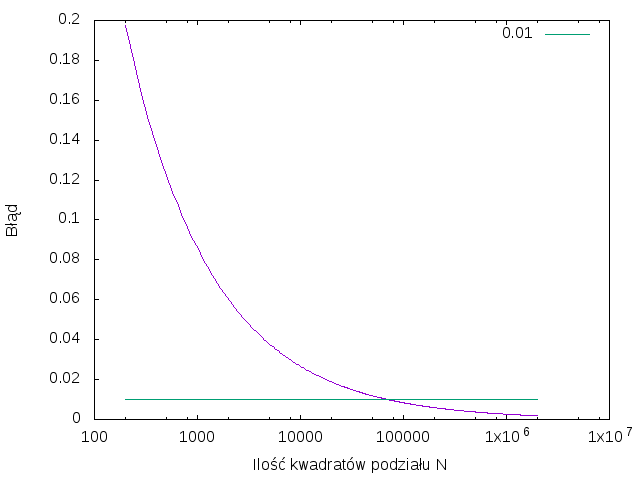
\includegraphics[width=0.7\textwidth]{PRST2.png}
\caption{Zależność błędu $\epsilon$ od ilości prostokątów $N$ na jakie podzielono obszar całkowania w metodzie prostokątów. 
	Linią poziomą zaznaczono błąd poniżej 0.01}\label{2}
\end{figure}
\begin{figure} 
\centering
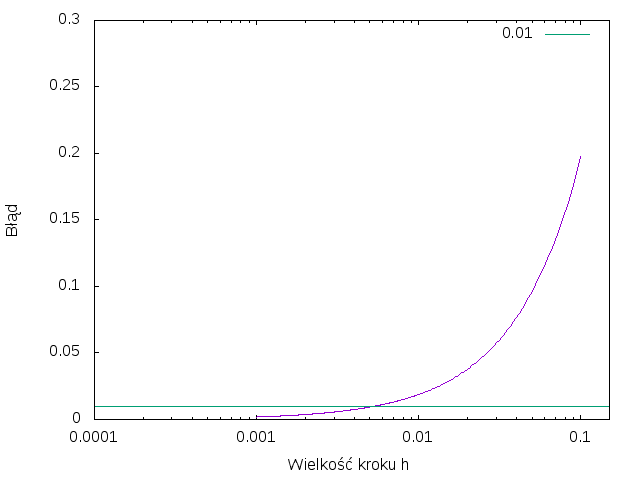
\includegraphics[width=0.7\textwidth]{PRST3.png}
\caption{Zależność błędu $\epsilon$ od długości podprzedziału $h$ metodzie prostokątów. 
	Linią poziomą zaznaczono błąd poniżej 0.01}\label{3}
\end{figure}
\section*{Podsumowanie}
Porównując wykresy \ref{1} i \ref{2} widzimy, iż metoda prostokątów szybciej (dla mniejszych $N$) daje wyniki obarczone małym błędem w przypadku
całkowania po obszarze dwuwymiarowym. Dla dopuszczalnego błędu rzędu 0.01 w metodzie prostokątów wystarczy $N=10^5$, natomiast dla metody
Monte Carlo jest to wielkość niewystarczająca. Wynik ten jest zgodny z przewidywaniem, gdyż metoda całkowania Monte Carlo jest lepsza od metody prostokątów
dopiero dla obszarów o wymiarze $d \ge 3$ [Źr. \cite{11}]. Widzimy również, że dla metody prostokątów uzyskana krzywa błędu jest gładka i monotoniczna.

\begin{thebibliography}{9}
\bibitem{11}
    \url{http://www.ftj.agh.edu.pl/~adamowski/wyklady_mofit_1/r3.pdf}
\end{thebibliography}



\end{document}


